\documentclass{article}
\usepackage{graphicx}
\usepackage{amssymb}
\usepackage{amsmath}
\usepackage{parskip}
\usepackage{tabularray}
\usepackage{tikz}
\usepackage[a4paper,margin=1.25cm]{geometry}

\newcounter{problem}
\newcounter{extraproblem}
\newcommand{\question}[1]{\refstepcounter{problem}\par\smallskip\textbf{T\theproblem.}\quad #1\par\smallskip}
\newcommand{\extraquestion}[1]{\refstepcounter{extraproblem}\par\smallskip\textbf{OT\theextraproblem.}\quad #1\par\smallskip}

\begin{document}
\title{Homework 4 Neural Networks}
\author{Nipat Chenthanakij 6430215121}
\date{}
\maketitle
\subsubsection*{T1. Compute the forward and backward pass of the given computation.}
\begin{align*}
    x_1 & =ReLU(x_0 w_0+b_0) \\
    y_1 & =x_1 w_1 + b_1     \\
    z   & =ReLU(y_1+x_0)
\end{align*}

\tikzset{every picture/.style={line width=0.75pt}} %set default line width to 0.75pt        
\begin{center}

    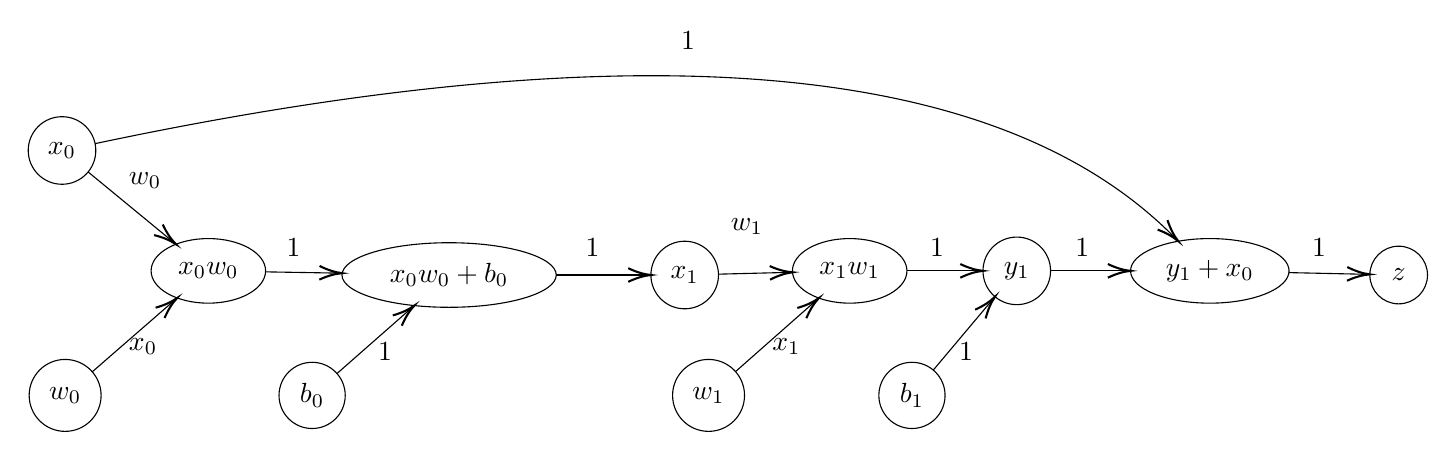
\begin{tikzpicture}[x=0.75pt,y=0.75pt,yscale=-1,xscale=1]
        %uncomment if require: \path (0,300); %set diagram left start at 0, and has height of 300
        % Text Node
        \draw    (51.5, 219) circle [x radius= 17.33, y radius= 17.33]   ;
        \draw (51.5,219) node   [align=left] {$\displaystyle w_{0}$};
        % Text Node
        \draw    (50, 101) circle [x radius= 16.28, y radius= 16.28]   ;
        \draw (50,101) node   [align=left] {$\displaystyle x_{0}$};
        % Text Node
        \draw    (120.5, 159) circle [x radius= 27.58, y radius= 15.56]   ;
        \draw (120.5,159) node   [align=left] {$\displaystyle x_{0} w_{0}$};
        % Text Node
        \draw    (236.5, 161) circle [x radius= 51.62, y radius= 15.56]   ;
        \draw (236.5,161) node   [align=left] {$\displaystyle x_{0} w_{0} +b_{0}$};
        % Text Node
        \draw    (170.5, 219) circle [x radius= 15.95, y radius= 15.95]   ;
        \draw (170.5,219) node   [align=left] {$\displaystyle b_{0}$};
        % Text Node
        \draw    (350, 161) circle [x radius= 16.28, y radius= 16.28]   ;
        \draw (350,161) node   [align=left] {$\displaystyle x_{1}$};
        % Text Node
        \draw    (361.5, 219) circle [x radius= 17.33, y radius= 17.33]   ;
        \draw (361.5,219) node   [align=left] {$\displaystyle w_{1}$};
        % Text Node
        \draw    (429.5, 159) circle [x radius= 27.58, y radius= 15.56]   ;
        \draw (429.5,159) node   [align=left] {$\displaystyle x_{1} w_{1}$};
        % Text Node
        \draw    (510, 159) circle [x radius= 16.28, y radius= 16.28]   ;
        \draw (510,159) node   [align=left] {$\displaystyle y_{1}$};
        % Text Node
        \draw    (459.5, 219) circle [x radius= 15.95, y radius= 15.95]   ;
        \draw (459.5,219) node   [align=left] {$\displaystyle b_{1}$};
        % Text Node
        \draw    (603, 159) circle [x radius= 38.18, y radius= 15.56]   ;
        \draw (603,159) node   [align=left] {$\displaystyle y_{1} +x_{0}$};
        % Text Node
        \draw    (694, 161) circle [x radius= 13.89, y radius= 13.89]   ;
        \draw (694,161) node   [align=left] {$\displaystyle z$};
        % Text Node
        \draw (81,110.4) node [anchor=north west][inner sep=0.75pt]    {$w_{0}$};
        % Text Node
        \draw (81,190.4) node [anchor=north west][inner sep=0.75pt]    {$x_{0}$};
        % Text Node
        \draw (157,142.4) node [anchor=north west][inner sep=0.75pt]    {$1$};
        % Text Node
        \draw (201,192.4) node [anchor=north west][inner sep=0.75pt]    {$1$};
        % Text Node
        \draw (301,142.4) node [anchor=north west][inner sep=0.75pt]    {$1$};
        % Text Node
        \draw (371,132.4) node [anchor=north west][inner sep=0.75pt]    {$w_{1}$};
        % Text Node
        \draw (391,190.4) node [anchor=north west][inner sep=0.75pt]    {$x_{1}$};
        % Text Node
        \draw (467,142.4) node [anchor=north west][inner sep=0.75pt]    {$1$};
        % Text Node
        \draw (481,192.4) node [anchor=north west][inner sep=0.75pt]    {$1$};
        % Text Node
        \draw (537,142.4) node [anchor=north west][inner sep=0.75pt]    {$1$};
        % Text Node
        \draw (347,42.4) node [anchor=north west][inner sep=0.75pt]    {$1$};
        % Text Node
        \draw (651,142.4) node [anchor=north west][inner sep=0.75pt]    {$1$};
        % Connection
        \draw    (62.57,111.34) -- (103.36,144.9) ;
        \draw [shift={(104.9,146.17)}, rotate = 219.44] [color={rgb, 255:red, 0; green, 0; blue, 0 }  ][line width=0.75]    (10.93,-3.29) .. controls (6.95,-1.4) and (3.31,-0.3) .. (0,0) .. controls (3.31,0.3) and (6.95,1.4) .. (10.93,3.29)   ;
        % Connection
        \draw    (64.58,207.63) -- (103.98,173.36) ;
        \draw [shift={(105.49,172.05)}, rotate = 138.99] [color={rgb, 255:red, 0; green, 0; blue, 0 }  ][line width=0.75]    (10.93,-3.29) .. controls (6.95,-1.4) and (3.31,-0.3) .. (0,0) .. controls (3.31,0.3) and (6.95,1.4) .. (10.93,3.29)   ;
        % Connection
        \draw    (148.06,159.48) -- (182.96,160.08) ;
        \draw [shift={(184.96,160.11)}, rotate = 180.99] [color={rgb, 255:red, 0; green, 0; blue, 0 }  ][line width=0.75]    (10.93,-3.29) .. controls (6.95,-1.4) and (3.31,-0.3) .. (0,0) .. controls (3.31,0.3) and (6.95,1.4) .. (10.93,3.29)   ;
        % Connection
        \draw    (182.48,208.47) -- (218.25,177.04) ;
        \draw [shift={(219.75,175.72)}, rotate = 138.69] [color={rgb, 255:red, 0; green, 0; blue, 0 }  ][line width=0.75]    (10.93,-3.29) .. controls (6.95,-1.4) and (3.31,-0.3) .. (0,0) .. controls (3.31,0.3) and (6.95,1.4) .. (10.93,3.29)   ;
        % Connection
        \draw    (288.12,161) -- (331.72,161) ;
        \draw [shift={(333.72,161)}, rotate = 180] [color={rgb, 255:red, 0; green, 0; blue, 0 }  ][line width=0.75]    (10.93,-3.29) .. controls (6.95,-1.4) and (3.31,-0.3) .. (0,0) .. controls (3.31,0.3) and (6.95,1.4) .. (10.93,3.29)   ;
        % Connection
        \draw    (366.27,160.59) -- (399.95,159.74) ;
        \draw [shift={(401.95,159.69)}, rotate = 178.56] [color={rgb, 255:red, 0; green, 0; blue, 0 }  ][line width=0.75]    (10.93,-3.29) .. controls (6.95,-1.4) and (3.31,-0.3) .. (0,0) .. controls (3.31,0.3) and (6.95,1.4) .. (10.93,3.29)   ;
        % Connection
        \draw    (374.49,207.54) -- (413.14,173.43) ;
        \draw [shift={(414.64,172.11)}, rotate = 138.58] [color={rgb, 255:red, 0; green, 0; blue, 0 }  ][line width=0.75]    (10.93,-3.29) .. controls (6.95,-1.4) and (3.31,-0.3) .. (0,0) .. controls (3.31,0.3) and (6.95,1.4) .. (10.93,3.29)   ;
        % Connection
        \draw    (457.08,159) -- (491.72,159) ;
        \draw [shift={(493.72,159)}, rotate = 180] [color={rgb, 255:red, 0; green, 0; blue, 0 }  ][line width=0.75]    (10.93,-3.29) .. controls (6.95,-1.4) and (3.31,-0.3) .. (0,0) .. controls (3.31,0.3) and (6.95,1.4) .. (10.93,3.29)   ;
        % Connection
        \draw    (469.77,206.8) -- (498.23,172.98) ;
        \draw [shift={(499.52,171.45)}, rotate = 130.09] [color={rgb, 255:red, 0; green, 0; blue, 0 }  ][line width=0.75]    (10.93,-3.29) .. controls (6.95,-1.4) and (3.31,-0.3) .. (0,0) .. controls (3.31,0.3) and (6.95,1.4) .. (10.93,3.29)   ;
        % Connection
        \draw    (526.28,159) -- (562.82,159) ;
        \draw [shift={(564.82,159)}, rotate = 180] [color={rgb, 255:red, 0; green, 0; blue, 0 }  ][line width=0.75]    (10.93,-3.29) .. controls (6.95,-1.4) and (3.31,-0.3) .. (0,0) .. controls (3.31,0.3) and (6.95,1.4) .. (10.93,3.29)   ;
        % Connection
        \draw    (641.13,159.84) -- (678.11,160.65) ;
        \draw [shift={(680.11,160.69)}, rotate = 181.26] [color={rgb, 255:red, 0; green, 0; blue, 0 }  ][line width=0.75]    (10.93,-3.29) .. controls (6.95,-1.4) and (3.31,-0.3) .. (0,0) .. controls (3.31,0.3) and (6.95,1.4) .. (10.93,3.29)   ;
        % Connection
        \draw    (65.94,97.7) .. controls (328.66,42.1) and (502.2,57.34) .. (586.56,143.42) ;
        \draw [shift={(587.82,144.72)}, rotate = 226.12] [color={rgb, 255:red, 0; green, 0; blue, 0 }  ][line width=0.75]    (10.93,-3.29) .. controls (6.95,-1.4) and (3.31,-0.3) .. (0,0) .. controls (3.31,0.3) and (6.95,1.4) .. (10.93,3.29)   ;

    \end{tikzpicture}
\end{center}

Forward pass:
\begin{align*}
    x_1 & =ReLU(x_0w_0+b_0)  =ReLU(1(0.3)+0.1)  =0.4   \\
    y_1 & =x_1w_1+b_1        =0.4(-0.2)+(-0.3)  =-0.38 \\
    z   & =ReLU(y_1+x_0)     =ReLu(-0.38+1)     =0.62  \\
\end{align*}

Backward pass: We can compute the gradients using chain rule according to the computation graph shown above, where each edge is assigned the partial derivative w.r.t. the incoming node.
\begin{align*}
    \frac{\partial z}{\partial w_0} & =1(1)(1)(w_1)(1)(1)(x_0)=-0.2 \\
    \frac{\partial z}{\partial b_0} & =1(1)(1)(w_1)(1)(1)=-0.2      \\
    \frac{\partial z}{\partial w_1} & =1(1)(1)(x_1)=0.4             \\
    \frac{\partial z}{\partial b_1} & =1(1)(1)=1                    \\
\end{align*}

\subsubsection*{T2. Given the network architecture specifications, determine the size of the output A, B, and C.}
A has the output size of \(32 \times 1024\). B has the output size of \(32 \times 512\). And, C has the output size of \(32 \times 1\).

\subsubsection*{T3. What is the total number of learnable parameters in this network?}
The first layer has \(1024 \times 30 + 1024\) parameters (Weight and bias are included in the first and second term respectively). The second layer has \(512\times1024+512\) parameters. The last layer has \(512+1\) parameters.
Thus the network has a total of \(557,057\) learnable parameters.
\newpage
\subsubsection*{T4. Prove that the derivative of the loss w.r.t \(h_i\) is \(P(y=i)-y_i\).}
Let \(p_i=P(y=i)=\dfrac{e^{h_i}}{\sum_k e^{h_k}}\), we will calculate the derivative of \(p_j\) w.r.t. \(h_i\) in two cases where \(i=j\) and \(i\neq j\).

Case I: \(i\neq j\)
\begin{align*}
    \frac{\partial p_j}{\partial h_i} & =\frac{e^{h_j}\frac{\partial h_j}{\partial h_i} \sum_k e^{h_k}-e^{h_j}\sum_k{\frac{\partial (e^{h_k})}{\partial h_i}}}{\left( \sum_k e^{h_k} \right)^2} \\
                                      & =\frac{-e^{h_i}e^{h_j}}{\left( \sum_k e^{h_k} \right)^2}                                                                                                \\
                                      & =-p_i p_j
\end{align*}

Case II: \(i=j\)
\begin{align*}
    \frac{\partial p_i}{\partial h_i} & =\frac{e^{h_i}\frac{\partial h_i}{\partial h_i} \sum_k e^{h_k}-e^{h_i}\sum_k{\frac{\partial (e^{h_k})}{\partial h_i}}}{\left( \sum_k e^{h_k} \right)^2} \\
                                      & =\frac{e^{h_i}\sum_k e^{h_k}-e^{h_i}e^{h_i}}{\left( \sum_k e^{h_k} \right)^2}                                                                           \\
                                      & =p_i(1-p_i)
\end{align*}

The loss function is defined as \(L=-\sum_i y_i \log p_i\).
\begin{align*}
    \frac{\partial L}{\partial h_i} & = \frac{\partial}{\partial h_i}\left( -\sum_j y_j \log(p_j) \right)       \\
                                    & = -\sum_j y_j \frac{\partial}{\partial h_i}\log(p_j)                      \\
                                    & = -\sum_j \frac{y_j}{p_j}\frac{\partial p_j}{\partial h_i}                \\
                                    & = -\sum_{j\neq i} \frac{y_j}{p_j} (-p_i p_j) - \frac{y_i}{p_i} p_i(1-p_i) \\
                                    & = p_i \sum_{j\neq i} y_j - y_i + y_i p_i\\
                                    &= p_i \sum_k y_k - y_i\\
                                    &= p_i-y_i \quad \square
\end{align*}
\end{document}